\section{Generating referring expressions} \label{sec:gre}

We can connect description logics to the problem of generating
referring expressions via the concept of \emph{bisimulation classes}.
A bisimulation class is a maximal subset $C$ of the domain such that
all members of $C$ are pairwise bisimilar.  For the finite models we
deal with in GRE, this amounts to saying that there are certain
concepts that are satisfied by all individuals in $C$ and no
individuals that are not in $C$ (by Theorems~\ref{bisim} and
\ref{bisim2}).  If we represent referring expressions as DL concepts,
this means that there exists a unique referring expression for some
individual $a$ iff $a$ is alone in its bisimulation class; and if it
is, we can use one of the concepts that are characteristic for $C$ as
the referring expression.

Representing referring expressions as DL concepts is a very natural
perspective.  The purely conjunctive bag of propositional symbols that
e.g.\ \newcite{Dale1995} compute is clearly a conjunction in
description logic.  Relational expressions as in
\newcite{dale91:_gener_refer_expres_invol_relat} or
\newcite{Krahmer2003} are simply concepts of \el; for instance, ``the
book on the table'' corresponds to the concept $\mathsf{book} \sqcap
\exists \mathsf{on}. \mathsf{table}$.  And other propositional
connectives, such as disjunction and negation
\cite{deemter01:_gener_refer_expres}, can clearly be represented in
\alc\ as well.

All this means that we can reduce the problem of computing a unique RE
to the problem of computing the bisimulation classes of a model.  We
will now present two algorithms -- one for \alc\ and one for \el\ --
for doing this.  In fact, each of these algorithms computes all
bisimulation classes of a model at once, effectively computing a RE
for every single individual in the domain simultaneously.


\subsection{Bisimulation classes for \alc}


\subsection{Bisimulation classes for \el}

The algorithm we just presented is driven by case distinctions between
concepts $\varphi$ and $\neg \varphi$, and thus adds large amounts of
negations to the characteristic concepts.  This can be inconvenient
in NLG, because such concepts may be expressible only by rather clumsy
natural-language expressions. \todo{example?}  We will therefore
introduce a new algorithm which is limited to computing
(negation-free) concepts of \el.  

As before, the algorithm maintains a set $\C = \{C_1,\ldots,C_n\}$ of
concepts (this time of \el) such that $\interp{C_1} \cup \ldots \cup
\interp{C_n} = \Delta$, and which it refines iteratively.  However,
where the \alc\ algorithm maintains the invariant that
$\interp{C_1},\ldots,\interp{C_n}$ is a partition of $\Delta$, we
weaken this invariant to the requirement that there are no $m \geq 2$
pairwise different indices $1 \leq i_1,\ldots,i_m \leq n$ such that
$\interp{C_{i_1}} = \interp{C_{i_2}} \cup \ldots \cup
\interp{C_{i_m}}$.  We call the concept $C_{i_1}$ \emph{subsumed} if
such a decomposition exists.

\begin{algorithm}[t]
\dontprintsemicolon
\caption{\el\ bisimulation classes}
\label{algo:bisim-el}
$\C \leftarrow \{\top\}$ \;
\For{$p \in \prop$}{
  add$_\el$(p, \C) \;
}
\While{not all concepts in $\C$ singleton}{
  \For{$C \in \C$, $R \in \rel$}{
    add$_\el$($\exists R.C$, $\C$) \;
  }
  \If{made no changes to $\C$}{
    exit\;
  }
}
\end{algorithm}


\begin{algorithm}[t]
\dontprintsemicolon
\caption{add$_\el$($C$, $\C$)}
\label{algo:bisim-add-el}
\For{$C' \in \C$ non-singleton}{
  \If{$C' \sqcap C$ is not subsumed in $\C$}{
    add $C' \sqcap C$ to $\C$ \;
    remove subsumed concepts from $\C$\;
  }
}
\end{algorithm}

Algorithms~\ref{algo:bisim-el} and \ref{algo:bisim-add-el} compute
the \el\ bisimulation classes for a given model.
Algorithm~\ref{algo:bisim-el} iterates over all propositional and
relational symbols of the signature to construct new concepts until
either all concepts in $\C$ are singleton (i.e., there is only one
individual that satisfies them), or no progress has been made in the
previous iteration.  In each iteration, it calls the procedure
add$_\el$($C$, $\C$), which intersects $C$ with all current concepts
that are not already singleton, adds the result to $\C$ and then
removes all concepts in $\C$ that have become subsumed.  Removal of
subsumed concepts can be implemented efficiently by arranging the
concepts in $\C$ in a a graph that connects two concepts with an edge
if one is a maximal proper subset of the other.

\begin{figure}
  \centering
  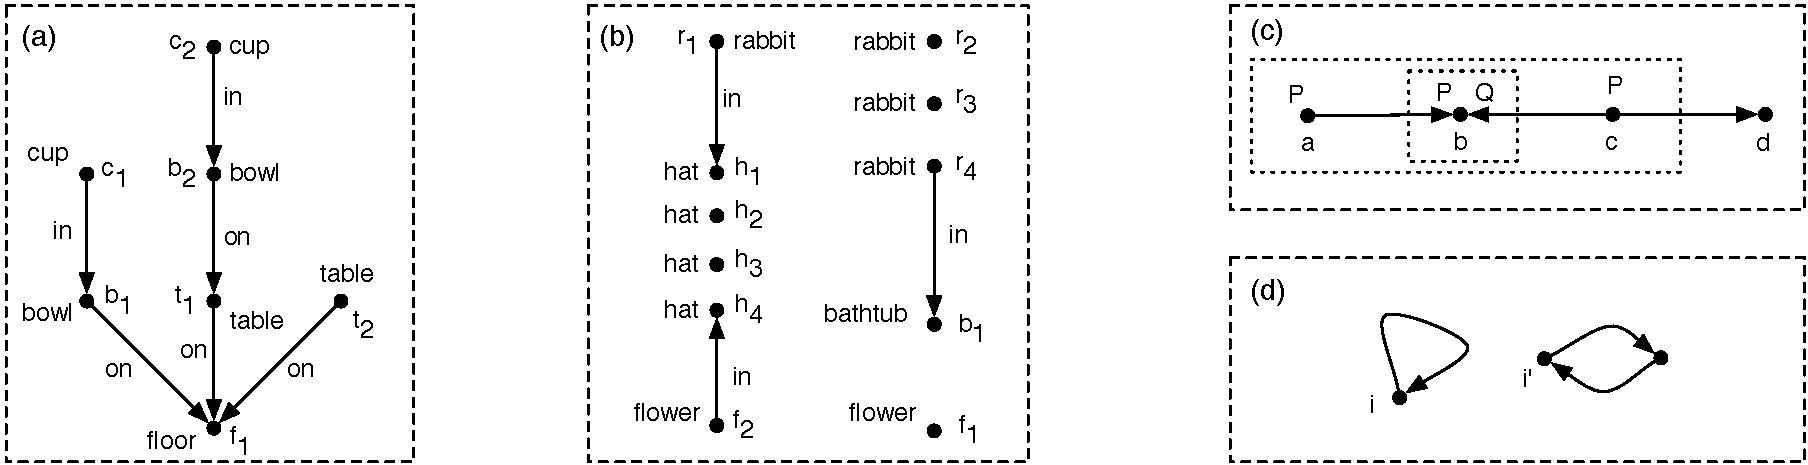
\includegraphics[width=5cm]{pic-dale-haddock}
  \caption{The Dale and Haddock scenario.}
  \label{fig:dale-haddock}
\end{figure}

\begin{figure}
  \centering
  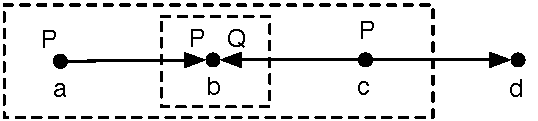
\includegraphics[width=\columnwidth]{pic-el-vs-alc}
  \caption{Illustrating the difference between \el\ and \alc.}
  \label{fig:el-vs-alc}
\end{figure}

Let's see what this algorithm does on the example shown in
Fig.~\ref{fig:dale-haddock}, which is taken from
\newcite{dale91:_gener_refer_expres_invol_relat}.  In the first loop,
the algorithm will add new concepts $\mathsf{floor}$, $\mathsf{bowl}$,
$\mathsf{cup}$, and $\mathsf{table}$; because adding these concepts
makes $\top$ subsumed, $\C$ will consist of these four concepts after
the loop.  Not all of these concepts are singleton; for instance,
$\interp{\mathsf{cup}}$ contains two individuals.  So we iterate over
the relations to make the concepts more precise.  After the first
iteration over the relations, we have $\C = \{ \mathsf{floor},
\mathsf{bowl} \sqcap \exists \mathsf{on}.\mathsf{floor}, \mathsf{bowl}
\sqcap \exists \mathsf{on}.\mathsf{table}, \mathsf{cup},
\mathsf{table} \}$. Notice that $\mathsf{bowl}$ has become subsumed,
but we haven't distinguished the cups and tables further, but we can
use the distinction between the bowls to distinguish the cups in the
second iteration.  The result of this is $\C = \{ \mathsf{floor},
\mathsf{bowl} \sqcap \exists \mathsf{on}.\mathsf{floor}, \mathsf{bowl}
\sqcap \exists \mathsf{on}.\mathsf{table}, \mathsf{cup} \sqcap \exists
\mathsf{in}. (\mathsf{bowl} \sqcap \exists
\mathsf{on}.\mathsf{floor}), \mathsf{cup} \sqcap \exists
\mathsf{in}. (\mathsf{bowl} \sqcap \exists
\mathsf{on}.\mathsf{table}), \mathsf{table} \}$.  At this point, all
concepts except for $\mathsf{table}$ are singleton, and further
iterations don't allow us to refine $\mathsf{table}$; so the algorithm
terminates.  Each of the singleton bisimulation classes is represented
by a characteristic concept; for instance, $\C$ tells us that
$\mathsf{cup} \sqcap \exists \mathsf{in}. (\mathsf{bowl} \sqcap
\exists \mathsf{on}.\mathsf{table})$ is only satisfied by $c_2$, so we
may refer to $c_2$ as ``the cup in the bowl on the table''.

Compared to the \alc\ algorithm, the \el\ algorithm will generally
compute larger bisimulation classes, and compute singleton
bisimulation classes less frequently, because the concepts it can
build can ``see'' fewer differences between individuals.  For example,
in the model shown in Fig.~\ref{fig:el-vs-alc}, the \alc\ algorithm
will compute the concepts $\{\neg \exists R. (\neg P \sqcap \neg Q),
\exists R. (\neg P \sqcap \neg Q), Q, \neg P \sqcap \neg Q\}$ (each of
which is singleton), but $a$ and $b$ are \el-bisimilar in this model,
and the only \el-concept that is true in $d$ is $\top$, so the \el\
algorithm can only compute the concepts $\{\top, P, P \sqcap Q\}$.
Furthermore, because the \el\ algorithm maintains a weaker invariant
for the classes, it may consider more of these classes simultaneously.
Prima facie, this means that it has worst-case exponential runtime,
given that the whole domain has an exponential number of subsets.
However, it is possible that a more careful analysis of the
combinatorics of the considered subsets reveal that the algorithm is
actually polynomial; it certainly behaves polynomially in our
evaluations (see below).


%%% Local Variables: 
%%% mode: latex
%%% TeX-master: "dl-gre-08"
%%% End: 
